\section{Scenario 2 - Curvature of the Earth}\label{sec:scenario2}
The purpose of this scenario is to show how the curvature of the Earth comes into play, as seen on the map in Figure \ref{fig:s2_map}. In this case, the UA starts near the GS and moves away from it in a somewhat straight line. To be mentioned that a PD controller is used in simulation of the UAS.

\begin{figure}[H]
	\hfill
	\subfigure[UAS Map Positioning]{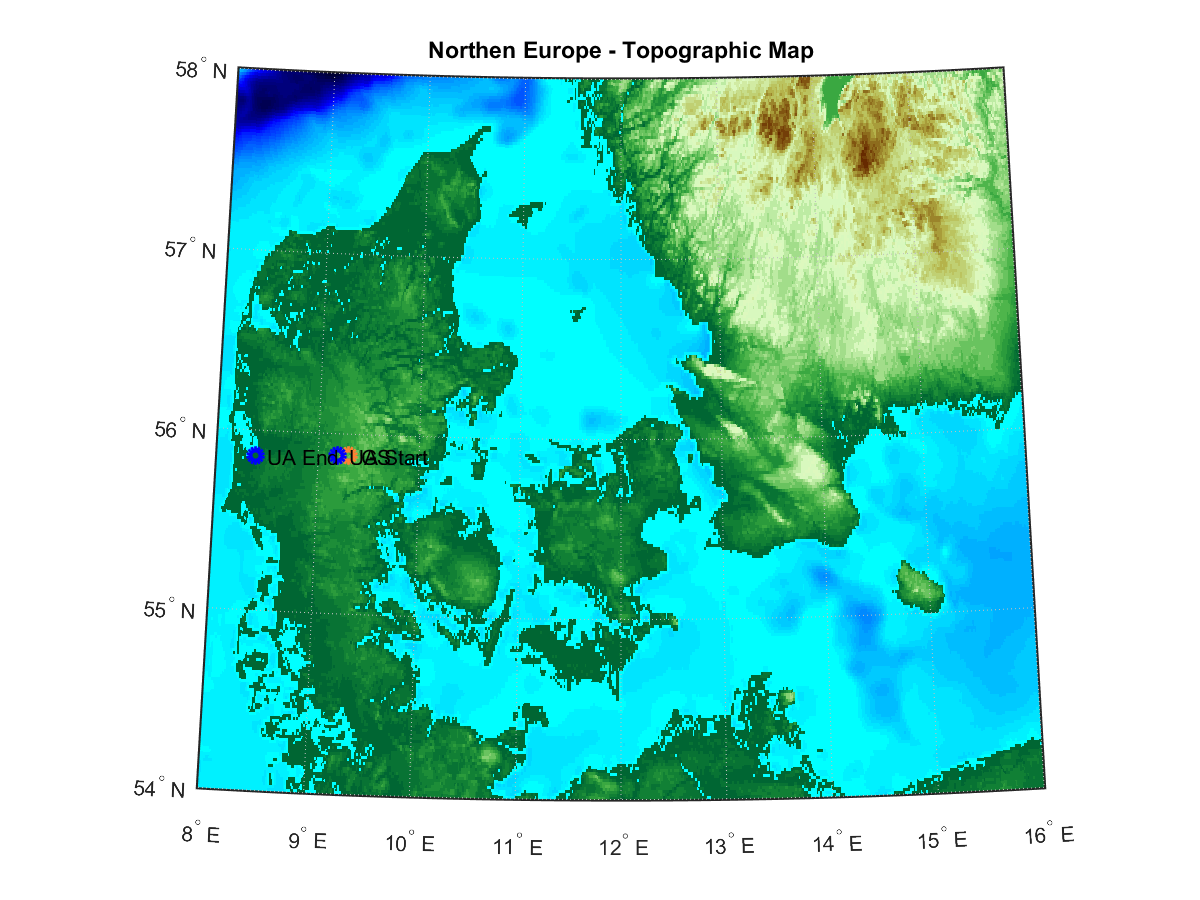
\includegraphics[scale=0.34]{figures/s2_map.png}}
	\hfill
	\subfigure[LOS and Distance]{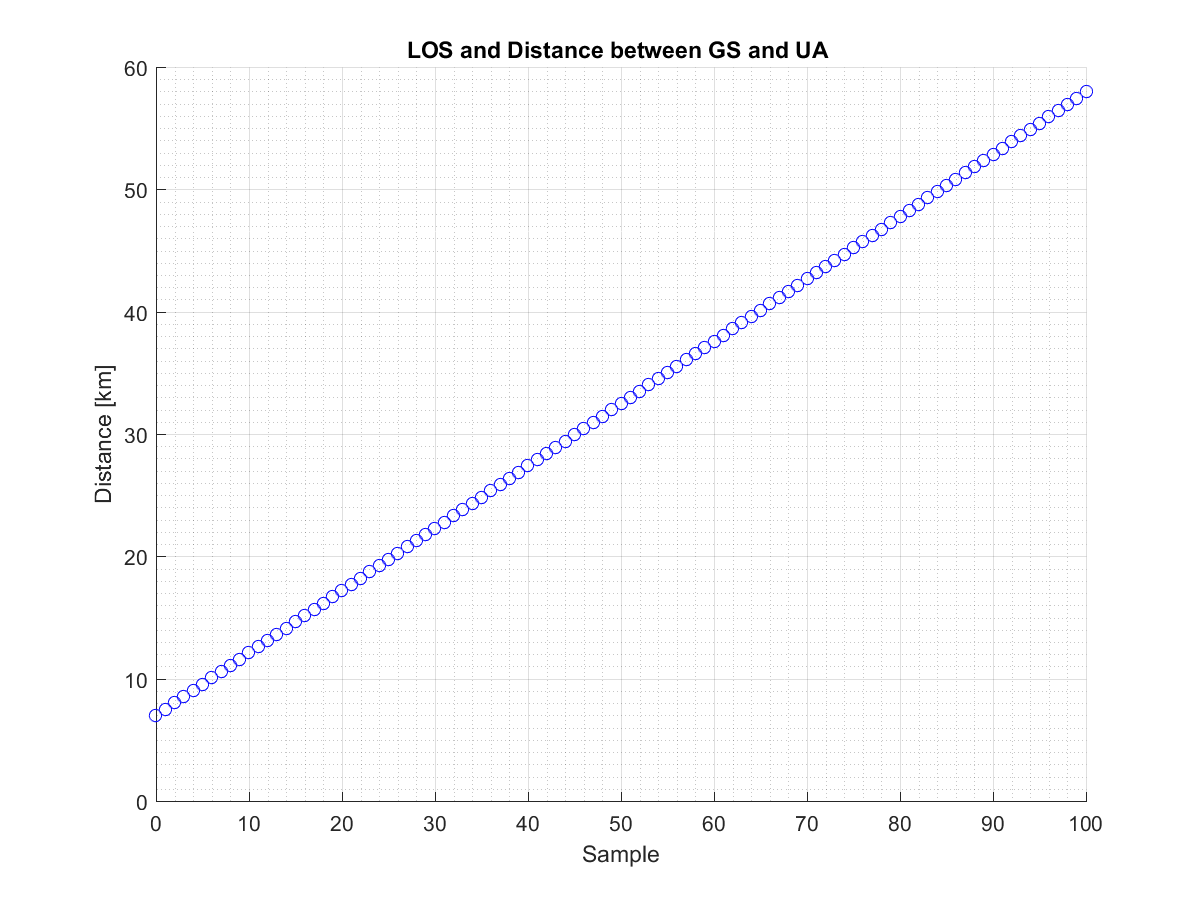
\includegraphics[scale=0.34]{figures/s2_los.png}}
	\hfill
	\caption{Mountain Scenario}
	\label{fig:s2_map}
\end{figure}


\subsection{Ground Station}
In this scenario, the UA is on the left side of the GS as is illustrated on Figure \ref{fig:s2_map}. As was explained in scenario 1, due to the chosen body frame coordinate of the GS, the optimal azimuth angle is always negative. On the other hand, the UA is flying away from the GS in a straight line which results in an almost constant azimuth angle. 

The optimal elevation angle has a slightly decrease (bigger than in the previous scenario) during the whole movement. It starts with a higher value because the UA is close to the GS. While the UA is progressing towards the end point, the distance between both devices grows which causes a decrease in the antenna's $\phi_{OPTIMAL}$ angle. However, in this situation, the $\phi_{OPTIMAL}$ becomes negative on the 70th sample, which means that, in the point of view of the GS, it has a bigger altitude compared to the UA one. The $\phi_{OPTIMAL}$ can achieve negative values because the curvature of the Earth was taken into account.

\begin{figure}[H]
	\centering
	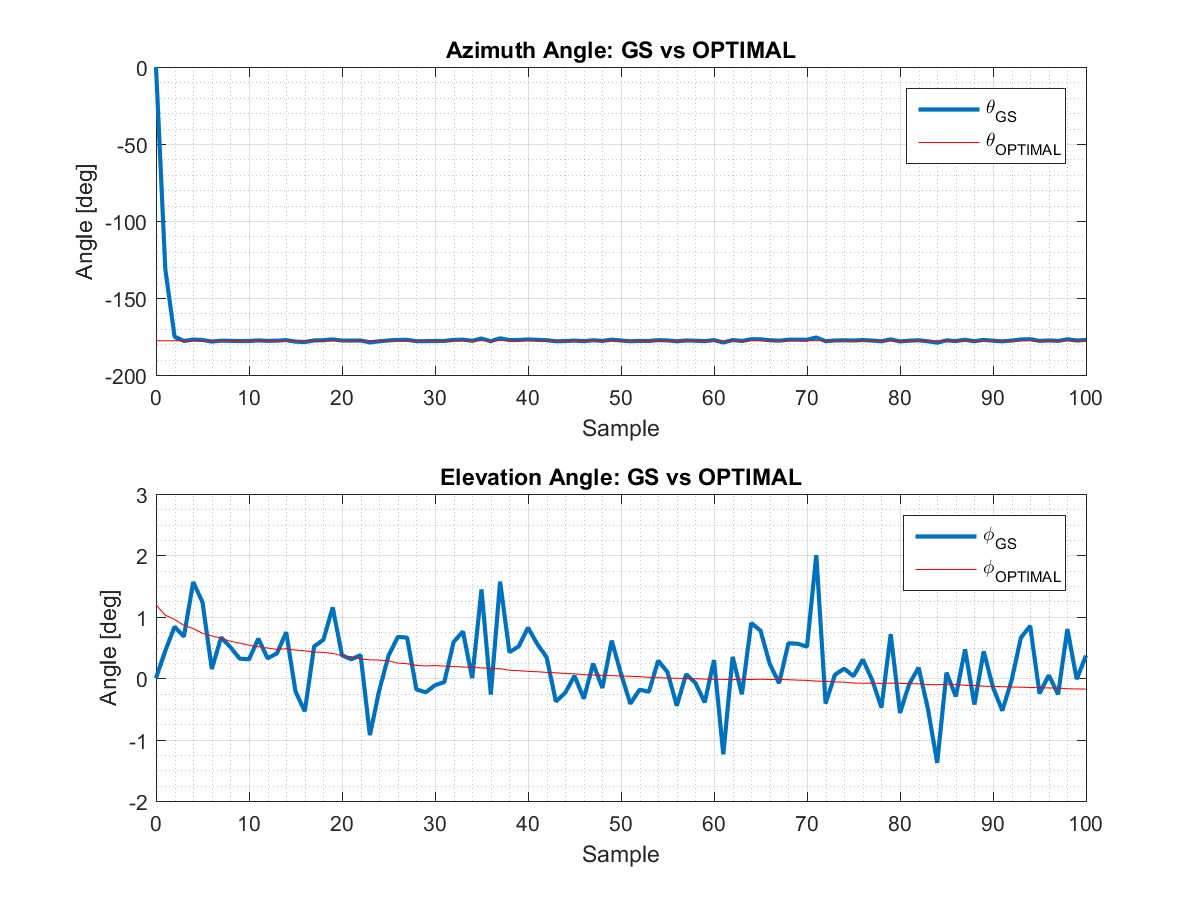
\includegraphics[scale=0.75]{figures/s2_gs.png}
	\caption{Azimuth and elevation angles of GS following the optimal angle}
	\label{fig:s2_gs}
\end{figure}

\subsection{Unmanned Aircraft}
The optimal elevation and Azimuth angle in Figure \ref{fig:s2_ua} has the same behaviour as the one in Figure \ref{fig:s2_gs} 

\begin{figure}[H]
	\centering
	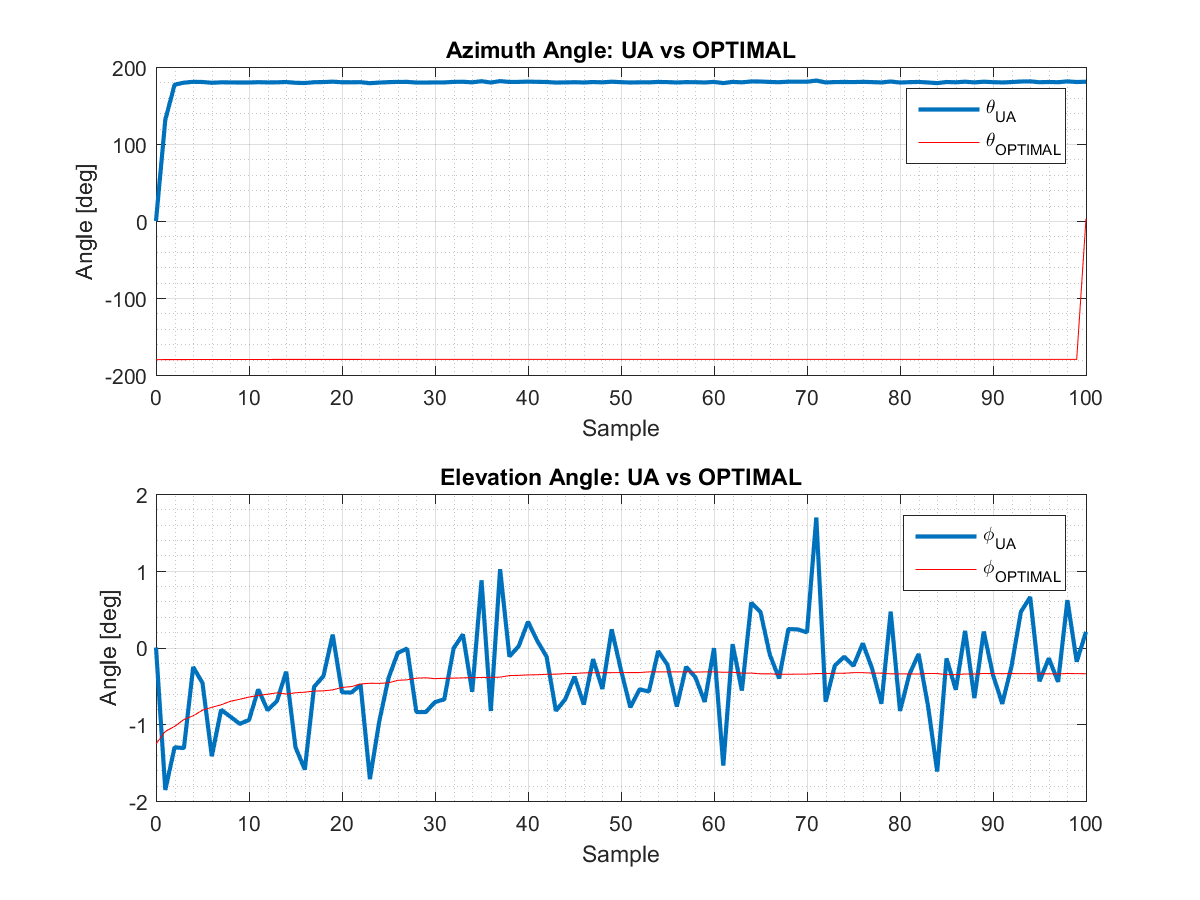
\includegraphics[scale=0.75]{figures/s2_ua.png}
	\caption{Azimuth and elevation angles of UA following the optimal angle}
	\label{fig:s2_ua}
\end{figure}


\subsection{Power}
In Figure \ref{fig:s2_power} the power at the receiver antenna of the GS antenna can be seen.

\begin{figure}[H]
	\centering
	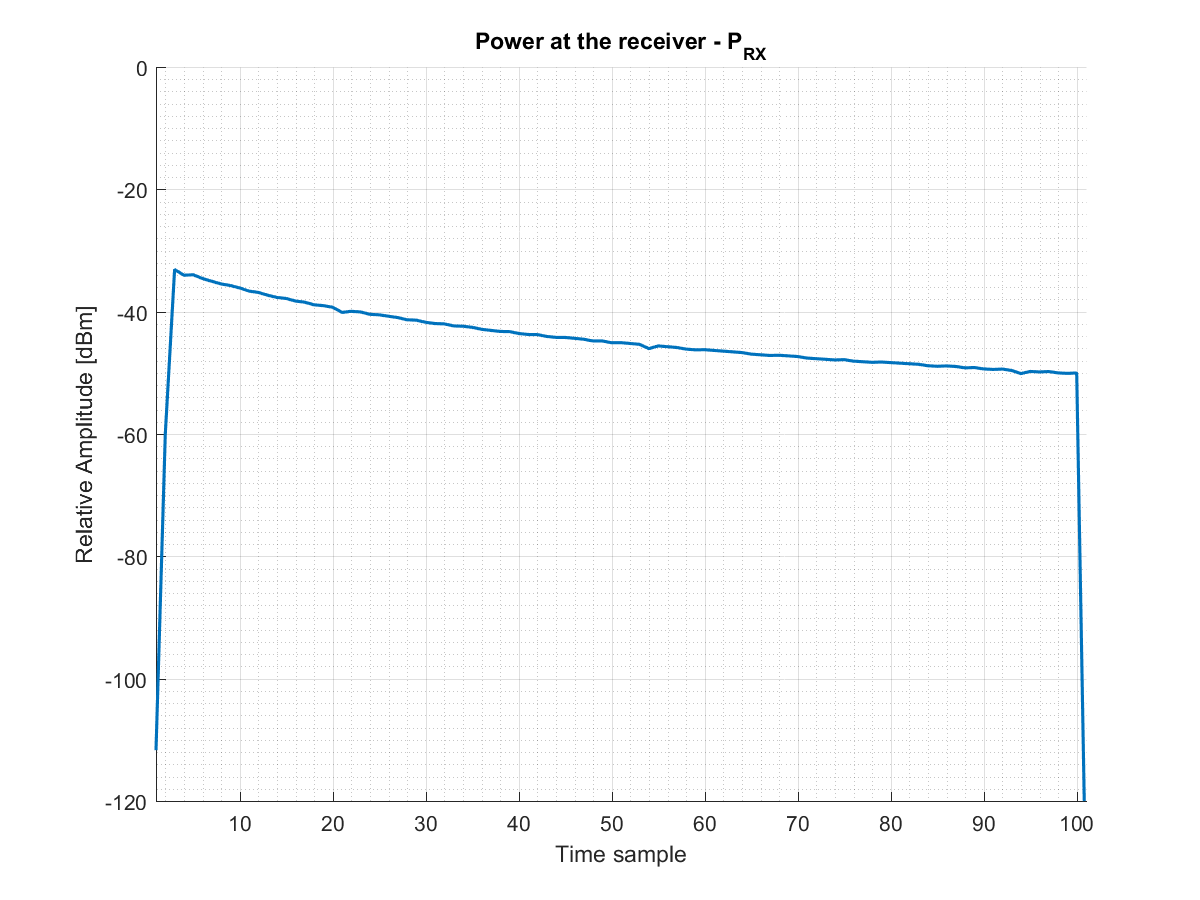
\includegraphics[scale=0.75]{figures/s2_power.png}
	\caption{Power at the receiver's antenna (GS)}
	\label{fig:s2_power}
\end{figure}

